
\begin{minipage}{0.49\textwidth}
\caption*{
tip pattern mode
}
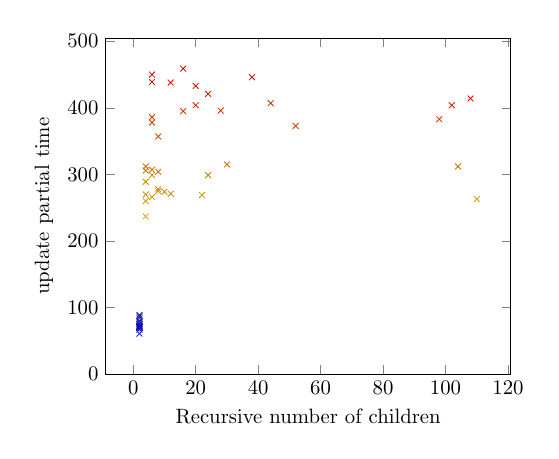
\begin{tikzpicture}[scale=0.75]
\begin{axis}[ymin=0, xlabel={Recursive number of children}, ylabel={update partial time}] \addplot[mark=x, color=blue, scatter, only marks] coordinates {
(2,67) (4,237) (2,61) (8,357) (10,274) (12,271) (2,71) (2,70) (6,450) (2,87) (2,80) (6,439) (8,304) (2,75) (2,70) (6,386) (16,395) (24,421) (38,446) (2,79) (4,270) (44,407) (2,73) (2,70) (4,306) (6,299) (8,275) (2,75) (4,289) (6,307) (16,459) (20,404) (22,269) (24,299) (2,70) (28,396) (30,315) (2,84) (4,312) (6,266) (2,79) (2,71) (2,71) (6,378) (8,278) (12,438) (20,433) (52,373) (98,383) (2,73) (102,404) (104,312) (2,89) (108,414) (110,263) (2,70) (4,260) };
\end{axis}
\end{tikzpicture}
\end{minipage}
\begin{minipage}{0.49\textwidth}
\caption*{
sites repeats mode
}
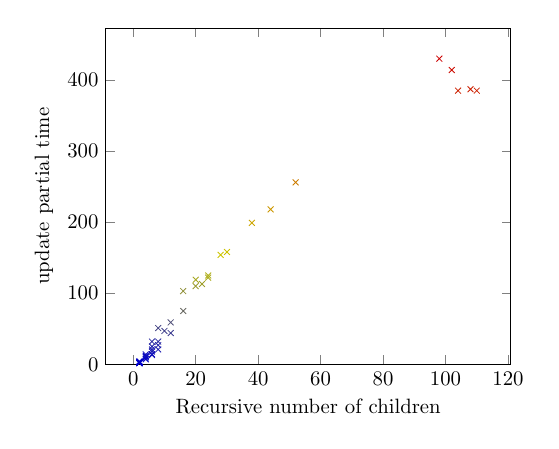
\begin{tikzpicture}[scale=0.75]
\begin{axis}[ymin=0, xlabel={Recursive number of children}, ylabel={update partial time}] \addplot[mark=x, color=blue, scatter, only marks] coordinates {
(2,4) (4,8) (2,2) (8,27) (10,47) (12,59) (2,2) (2,3) (6,18) (2,2) (2,2) (6,25) (8,32) (2,2) (2,2) (6,13) (16,75) (24,122) (38,199) (2,3) (4,11) (44,218) (2,3) (2,3) (4,14) (6,32) (8,51) (2,3) (4,10) (6,14) (16,103) (20,110) (22,113) (24,125) (2,3) (28,154) (30,158) (2,2) (4,12) (6,21) (2,4) (2,2) (2,2) (6,14) (8,21) (12,44) (20,119) (52,256) (98,430) (2,2) (102,414) (104,385) (2,3) (108,387) (110,385) (2,3) (4,7) };
\end{axis}
\end{tikzpicture}
\end{minipage}
